\section{Background}
\label{background}

The World-Wide Web (WWW), commonly known as the web, was invented to enable information sharing between remote collaborators and ''to be a pool of human knowledge'' \parencite[76]{BernersLeeCailliauLuotonenNielsenSecret1994}. The very first web page\footnote{http://info.cern.ch/hypertext/WWW/TheProject.html} was made available to the public in 1993 \hl{(ref)} and was written in HyperText Markup Language (HTML), which signature feature was the hyperlink \parencite{BernersLeeCailliauGroffPollermann1992}. The number of web pages published on the web grew fast. According to \textcite{BrinPage1998} World Wide Web Worm, one of the first search engines, had in 1994 110,000 pages in it's index. In 1997 the index of the top search engines at that time contained at least 2 million web pages \parencite{BrinPage1998}. \hl{how about today?} Today there are more than 1 billion web \emph{sites} on the web \hl{ref}, where each site contains at least one page, normally many many more. \hl{the definition of a page is no longer clear}. As will be described in the chapter on web apps the definition of a page is no longer an easy one to make.

In 1996 the W3C recommendation on Cascading Style Sheets (CSS) was published \parencite{LieBos1996}. \citeauthor{LieBos1996} describes CSS as a simple mechanism that ''allows authors and readers to attach style (e.g. fonts, colors and spacing) to HTML documents'' based on CSS rules \parencite*[1]{LieBos1996}. In parallel with the development of CSS, the development of JavaScript was also underway \parencite{Eich2011}.

JavaScript was intended to be used for simple tasks such as client-side form validation and \hl{one more example} \parencite{Zakai2018,Moller2018} but it's capabilities evolved and led to inventions such as manipulation of the Document Object Model (DOM) \parencite{WoodLeHorsApparaoByrneChampionIsaacsJacobsNicolRobieSutor1998} and Asynchronous JavaScript and XML (AJAX) \parencite{NielsonWilliamsonArlitt2008}.

The set of original web technologies was all introduced in just a few years in 1993 to 1996 as illustrated in Figure \ref{figure:webtechnologies-timeline}.

HTML, CSS, and JavaScript (Figure \ref{figure:webtechnologies-timeline}) are considered the core web technologies \parencite{MajchrzakBiornHansenGronli2018}.

% The last few years more advanced applications has moved to the web, mandating higher performance (REF).

% dynamiska webbsidor typ som första kapitel och att de i många fall lider av prestandaproblem, sätter upp varför vi behöver benchmarking.

\begin{comment}

\begin{figure}[!h]
\centering
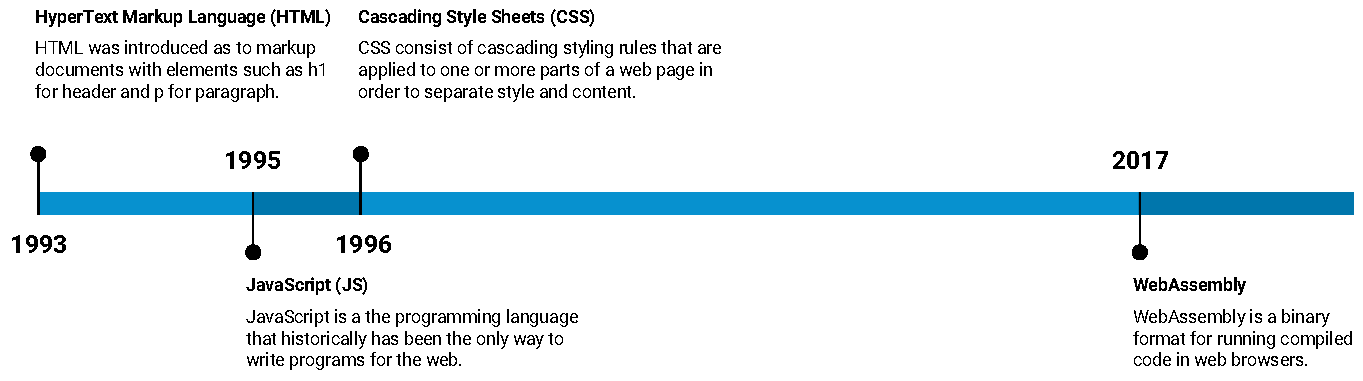
\includegraphics[width=16cm,keepaspectratio]{../Figures/webtechnologies-timeline}
\caption{Timeline of major web technologies: (a) HTML, (b) CSS, (c) JavaScript and it's newest member (d) WebAssembly.}
\label{figure:webtechnologies-timeline}
\end{figure}
    
\end{comment}

The introduction of JavaScript has thus lead the evolution of the web browser as a web page reader towards a platform for web applications \hl{ref}.

\subsection{Web apps}
\subfile{webapps}

\subsection{JavaScript}
\subfile{javascript}

\subsection{WebAssembly}
\subfile{webassembly}

\subsection{Benchmarking}
\subfile{benchmarking}
